\begin{frame}{(Re-)Validation of BeamPipeKiller}
    \begin{columns}
        \begin{column}{0.5\textwidth}
            \begin{figure}
                \centering
                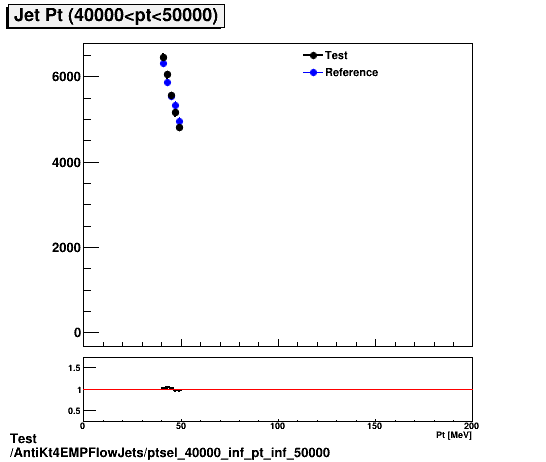
\includegraphics[width = \textwidth]{beam_highpT}
            \end{figure}
        \end{column}
        \begin{column}{0.5\textwidth}
            \begin{figure}
                \centering
                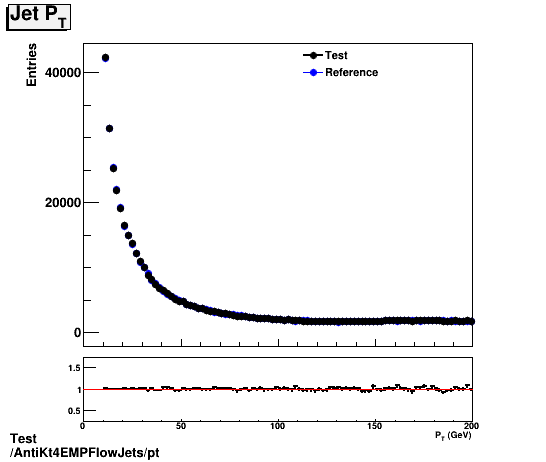
\includegraphics[width = \textwidth]{beam_pT}
            \end{figure}
        \end{column}
    \end{columns}
        \begin{itemize}
        \item \href{https://atlas-computing.web.cern.ch/atlas-computing/links/PhysValDir/JetEtMiss/jet_21-08-04_task1/AntiKt4EMPFlowJets/index.html}{EMPFlow}: High pT jets yellow
        \item \href{https://atlas-computing.web.cern.ch/atlas-computing/links/PhysValDir/JetEtMiss/jet_21-08-04_task1/AntiKt4EMTopoJets/index.html}{EMTopo}: green
        \item \href{https://atlas-computing.web.cern.ch/atlas-computing/links/PhysValDir/JetEtMiss/jet_21-08-04_task1/AntiKt4LCTopoJets/index.html}{LCTopo}: green
    \end{itemize}
\end{frame}